% Options for packages loaded elsewhere
\PassOptionsToPackage{unicode}{hyperref}
\PassOptionsToPackage{hyphens}{url}
\documentclass[12pt, ]{article}

\usepackage{mathtools}
\usepackage{amsmath}
\usepackage{amsthm}
\usepackage{amssymb}
\usepackage[italicdiff]{physics}
\mathtoolsset{showonlyrefs}

% SPACING AND FONTS %%%%%%%%%%%%%%%%%%%%%%%%%%%%%%%%%%%%%%%%%%%%%%%%%%%%%%%%%%%%
\usepackage{iftex}
% CAREFUL: the order of font includes here is very important!
\ifPDFTeX
  \usepackage[OT1,T1]{fontenc}
  \usepackage[utf8]{inputenc}
  \usepackage{textcomp} % provide euro and other symbols
    \usepackage[p,osf,swashQ]{cochineal}
  \usepackage[cochineal,vvarbb]{newtxmath}
      \usepackage[scale=0.95]{biolinum}
    \usepackage[scale=0.95,varl]{inconsolata}
\else % if luatex or xetex
  \usepackage[scale=0.95,varl]{inconsolata}
  \usepackage{newpxtext}
  \usepackage{mathpazo}
    \usepackage[scale=0.95]{biolinum}
  \fi
\ifLuaTeX
  \usepackage{selnolig}  % disable illegal ligatures
\fi
\IfFileExists{microtype.sty}{% use microtype if available
  \usepackage[]{microtype}
  \UseMicrotypeSet[protrusion]{basicmath} % disable protrusion for tt fonts
}{}

\setlength{\parindent}{0pt}
\setlength{\parskip}{10pt plus 2pt minus 2pt}
\setlength{\emergencystretch}{3em} % prevent overfull lines
\widowpenalty=10000
\clubpenalty=10000
\flushbottom
\allowdisplaybreaks
\sloppy


% CORE PACKAGES %%%%%%%%%%%%%%%%%%%%%%%%%%%%%%%%%%%%%%%%%%%%%%%%%%%%%%%%%%%%
\usepackage[dvipsnames,svgnames,x11names]{xcolor}
\usepackage[lmargin=1.5in,rmargin=1.5in,tmargin=1.2in,bmargin=1.2in]{geometry}
\usepackage[format=plain,
  labelfont={bf,sf,small,singlespacing},
  textfont={sf,small,singlespacing},
  justification=justified,
  margin=0.25in]{caption}

% SECTIONS AND HEADINGS %%%%%%%%%%%%%%%%%%%%%%%%%%%%%%%%%%%%%%%%%%%%%%%%%%%%%%%%
\setcounter{secnumdepth}{4}
\usepackage{sectsty}
\usepackage[compact]{titlesec}
% short title
\makeatletter
\newcommand\@shorttitle{}
\newcommand\shorttitle[1]{\renewcommand\@shorttitle{#1}}
\usepackage{fancyhdr}
\fancyhf{}
\pagestyle{fancy}
\renewcommand{\headrulewidth}{0pt}
\fancyheadoffset{0pt}
%\lhead{\scshape \@shorttitle}
%\rhead{\scshape\today}
\cfoot{\thepage}
\makeatother
% abstract styling
\renewenvironment{abstract}{
  \centerline
  {\large\sffamily\bfseries Abstract}\vspace{-1em}
  \begin{quote}\small
}{
  \end{quote}
}

% PANDOC INCLUDES %%%%%%%%%%%%%%%%%%%%%%%%%%%%%%%%%%%%%%%%%%%%%%%%%%%%%%%%%%%%%%

\providecommand{\tightlist}{%
  \setlength{\itemsep}{0pt}\setlength{\parskip}{0pt}}\usepackage{longtable,booktabs,array}
\usepackage{calc} % for calculating minipage widths
% Correct order of tables after \paragraph or \subparagraph
\usepackage{etoolbox}
\makeatletter
\patchcmd\longtable{\par}{\if@noskipsec\mbox{}\fi\par}{}{}
\makeatother
% Allow footnotes in longtable head/foot
\IfFileExists{footnotehyper.sty}{\usepackage{footnotehyper}}{\usepackage{footnote}}
\makesavenoteenv{longtable}
\usepackage{graphicx}
\makeatletter
\def\maxwidth{\ifdim\Gin@nat@width>\linewidth\linewidth\else\Gin@nat@width\fi}
\def\maxheight{\ifdim\Gin@nat@height>\textheight\textheight\else\Gin@nat@height\fi}
\makeatother
% Scale images if necessary, so that they will not overflow the page
% margins by default, and it is still possible to overwrite the defaults
% using explicit options in \includegraphics[width, height, ...]{}
\setkeys{Gin}{width=\maxwidth,height=\maxheight,keepaspectratio}
% Set default figure placement to htbp
\makeatletter
\def\fps@figure{htbp}
\makeatother
% END PANDOC %%%%%%%%%%%%%%%%%%%%%%%%%%%%%%%%%%%%%%%%%%%%%%%%%%%%%%%%%%%%%%%%%%%

% USER INCLUDES %%%%%%%%%%%%%%%%%%%%%%%%%%%%%%%%%%%%%%%%%%%%%%%%%%%%%%%%%%%%%%%%
% additional LaTeX code for the "preamble" goes here
\makeatletter
\makeatother
\makeatletter
\makeatother
\makeatletter
\@ifpackageloaded{caption}{}{\usepackage{caption}}
\AtBeginDocument{%
\ifdefined\contentsname
  \renewcommand*\contentsname{Table of contents}
\else
  \newcommand\contentsname{Table of contents}
\fi
\ifdefined\listfigurename
  \renewcommand*\listfigurename{List of Figures}
\else
  \newcommand\listfigurename{List of Figures}
\fi
\ifdefined\listtablename
  \renewcommand*\listtablename{List of Tables}
\else
  \newcommand\listtablename{List of Tables}
\fi
\ifdefined\figurename
  \renewcommand*\figurename{Figure}
\else
  \newcommand\figurename{Figure}
\fi
\ifdefined\tablename
  \renewcommand*\tablename{Table}
\else
  \newcommand\tablename{Table}
\fi
}
\@ifpackageloaded{float}{}{\usepackage{float}}
\floatstyle{ruled}
\@ifundefined{c@chapter}{\newfloat{codelisting}{h}{lop}}{\newfloat{codelisting}{h}{lop}[chapter]}
\floatname{codelisting}{Listing}
\newcommand*\listoflistings{\listof{codelisting}{List of Listings}}
\makeatother
\makeatletter
\@ifpackageloaded{caption}{}{\usepackage{caption}}
\@ifpackageloaded{subcaption}{}{\usepackage{subcaption}}
\makeatother
\makeatletter
\@ifpackageloaded{tcolorbox}{}{\usepackage[skins,breakable]{tcolorbox}}
\makeatother
\makeatletter
\@ifundefined{shadecolor}{\definecolor{shadecolor}{rgb}{.97, .97, .97}}
\makeatother
\makeatletter
\makeatother
\makeatletter
\makeatother
% END USER INCLUDES %%%%%%%%%%%%%%%%%%%%%%%%%%%%%%%%%%%%%%%%%%%%%%%%%%%%%%%%%%%%

% BIBLIOGRAPHY %%%%%%%%%%%%%%%%%%%%%%%%%%%%%%%%%%%%%%%%%%%%%%%%%%%%%%%%%%%%%%%%%
\usepackage[]{natbib}
\bibliographystyle{apalike}

% Give it this name so that it works with ::: #refs
\newenvironment{CSLReferences}[2]{
\bibliography{bibliography.bib}
\clearpage
}{}

% LINKS %%%%%%%%%%%%%%%%%%%%%%%%%%%%%%%%%%%%%%%%%%%%%%%%%%%%%%%%%%%%%%%%%%%%%%%%
\usepackage{hyperref}
\usepackage{url}
\hypersetup{
  pdftitle={Does EU Foreign Aid Cause Growth in the Short-Term? An Extension and Replication of Carnegie and Marinov (2017)},
  pdfauthor={David Alzate },
  colorlinks=true,
  linkcolor={black},
  filecolor={Maroon},
  citecolor={VioletRed4},
  urlcolor={DodgerBlue4},
  pdfcreator={LaTeX via pandoc}}

% TITLE, AUTHOR, DATE %%%%%%%%%%%%%%%%%%%%%%%%%%%%%%%%%%%%%%%%%%%%%%%%%%%%%%%%%%
\title{\sffamily\bfseries\huge\parfillskip=0pt
\rightskip=0pt plus .5\textwidth
\leftskip=0pt plus .5\textwidth
\emergencystretch=.3\textwidth Does EU Foreign Aid Cause Growth in the
Short-Term? An Extension and Replication of Carnegie and Marinov (2017)}
\shorttitle{Does EU Foreign Aid Cause Growth in the Short-Term? An Extension and Replication of Carnegie and Marinov (2017)}
\author{\textbf{David Alzate \footnote{Yale University. Replication
  files and code are available in
  \url{https://github.com/dalzatepro/aqrd-paper}}}
 }
\date{December 18, 2023}


\begin{document}
\allsectionsfont{\sffamily}

\maketitle

\begin{abstract}
Foreign aid from the EU and other ``Western'' sources continues to be a
sizable source of resources for low- and middle-income countries. Yet
the effects of aid on recipient countries' institutions and development
continues to be a topic of heated debate. Following
\citet{carnegie2017foreign}, I leverage variation in the rotating
presidency of the Council of the European Union to study the causal
effects of aid on growth. I find that increased EU aid does not have a
statistically significant positive impact on (log) GDP or GDP per capita
in the short-term (i.e., a four-year period), and find suggestive
evidence of a negative effect. I replicate \citet{carnegie2017foreign}'s
findings that EU aid leads to short-lived improvements in measures of
human rights and democracy.
\end{abstract}

\ifdefined\Shaded\renewenvironment{Shaded}{\begin{tcolorbox}[interior hidden, boxrule=0pt, borderline west={3pt}{0pt}{shadecolor}, enhanced, frame hidden, sharp corners, breakable]}{\end{tcolorbox}}\fi



% USER BODY %%%%%%%%%%%%%%%%%%%%%%%%%%%%%%%%%%%%%%%%%%%%%%%%%%%%%%%%%%%%%%%%%%%%

\hypertarget{introduction}{%
\section{Introduction}\label{introduction}}

Foreign aid -- or Overseas Development Assistance (ODA) -- has been a
stable source of financing for low- and middle-income countries since
aid flows began in the aftermath of World War II \citep{ahmad2020six}.
While low- and middle-income countries have other sources of development
financing, ODA continues to be a stable and sizable source of resources
\citep{ahmad2020six}. ``Western'' aid -- or ODA from OECD members,
including the EU -- is still larger than ``non-Western'' aid from
non-OECD members such as China. International development cooperation
funds in China reached USD 4.4 billion in 2019, compared to 152.8
billion by members of the OECD's Development Assistance Committee
\citep{ahmad2020six}.

The effects of aid, and particularly ``Western'' aid, on recipient
countries continues to be a topic of heated debate. Some scholars argue
that aid has the potential to unlock economic growth and development in
recipient countries (e.g., \citet{sachs2005end}). Others argue aid has a
pernicious effect as it can breed corruption, create dependencies,
impose agendas that do not cause growth in recipient countries, and
crowd-out domestic development
\citep{easterly2006white, pritchett2015can}. Yet it is hard to determine
the causal effects of aid on development. Aid might affect development
by changing local institutions and politics, by changing productivity
and economic activity, a combination both, or through other effects.
Most studies about the effects of aid have relied on cross-country data
and associations \citep{edwards2014economic}, which makes it difficult
to assess any causal claims and disentangle mechanisms.

One cross-country study that goes beyond associations and aims to make a
causal claim is \citet{carnegie2017foreign}. These authors study the
effects of EU aid on indicators of human rights and democracy in
recipient countries. They are able to isolate the causal effects of aid
by leveraging as-if-random variation from the rotating presidency of the
Council of the European Union. Using an instrumental variables approach,
they find EU Council presiding countries allocate significantly more aid
to their former colonies. This increased aid, in turn, has positive
effects on human rights and democracy, although ``the effects are
short-lived after the shock to aid dissipates''
\citep{carnegie2017foreign}.

If ``Western'' aid appears to have positive, albeit temporary, effects
on democracy and human rights, does it also affect economic growth?
Scholars argue that democracy and development are connected:
\citet{acemoglu2019democracy} find democracy has a positive effect on
GDP per capita. Yet the effects of democracy on growth might take time
to materialize; short-lived improvements on democracy might not suffice
to bring about growth. Aid might also improve economic growth even if it
has limited effects on democracy and human rights, for example, by
investing in capital that enhances productivity in recipient countries.
On the other hand, aid might disincentivize local growth if it leads to
the types of dependencies and corruption that aid detractors warn about.

Following \citet{carnegie2017foreign}, I leverage variation in the
rotating presidency of the Council of the European Union to study the
effects of aid on growth. I find that increased EU aid does not have a
statistically significant impact on (log) GDP or GDP per capita in the
short-term (i.e., a four-year period). If anything, I find suggestive
evidence that EU aid leads to a slight decrease in GDP growth in the
short term. I also replicate \citet{carnegie2017foreign}'s original
findings about aid's impact on democracy and human rights.

This paper is organized as follows. Section 2 describes the details of
my data and methods. Section 3 replicates \citet{carnegie2017foreign}'s
results and extends them to include (log) GDP and GDP per capita as
outcome variables. Section 4 concludes.

\hypertarget{data-and-methods}{%
\section{Data and Methods}\label{data-and-methods}}

To isolate the effects of EU foreign aid on economic growth over the
short-term, I \citet{carnegie2017foreign}'s instrumental variables
approach. The Presidency of the EU Council rotates every six months
among member states, based on alphabetical order. The country presiding
the Council has influence over the EU foreign aid budget. For historical
and political reasons, the presiding country might decide aid
allocations in favor of countries that used to be its former
colonies.\footnote{For details on how this rotating presidency works,
  please refer to \citet{carnegie2017foreign}} This as-if-random
variation in who allocates EU foreign aid can be used as an instrument
to isolate the effects of aid itself. The instrument, in this case, is
defined as \(Colony_{i(t-2)}\), an indicator variable that equals one
when an aid recipient country is a former colony of the country
presiding the EU Council in the second half of the year \(t-2\).

The relationship between \(Colony_{i(t-2)}\) and foreign aid is defined
by the following first-stage equation:

\begin{equation}\protect\hypertarget{eq-first}{}{
log(ODA)_{i(t-1)} = \gamma_{0} + \gamma_{1}Colony_{i(t-2)} + u_{it}
}\label{eq-first}\end{equation}

Where log(ODA) is the logarithm of the amount of EU aid a country \(i\)
received in year \(t-1\), and \(u_{it}\) is an error term.

We can expand on this first-stage equation by adding country-level and
year-level fixed effects. While these are not necessary to isolate the
first-stage relationship between \(Colony_{i(t-2)}\) and
\(log(ODA)_{i(t-1)}\) , they can help add precision by reducing sampling
variability \citep{carnegie2017foreign}. Adding fixed effects controls
for the time-invariant characteristics within each foreign aid recipient
country (such as geography), as well as the country-invariant
characteristics across years (such as global shocks that affected all
countries). These effects are shown in the equation below:

\begin{equation}\protect\hypertarget{eq-firstFE}{}{
log(ODA)_{i(t-1)} = \gamma_{0} + \gamma_{1}Colony_{i(t-2)} + \Sigma_{k \in K} \beta_{k}I(i=k) +\Sigma_{j \in j} \beta_{j}I(t=j) + u_{it}
}\label{eq-firstFE}\end{equation}

\(\Sigma_{k \in K} \beta_{k}I(i=k)\) stands for country-level fixed
effects; \(\Sigma_{j \in j} \beta_{j}I(t=j)\) stands for year-level
fixed effects.

For this instrument to be valid, it must be the case that (i) the
rotating presidency of the EU Council must be randomly assigned; (ii)
the rotating presidency of the EU Council affects the amount of EU
foreign aid allocated to recipient countries (i.e., \(\gamma_{1}\) must
be nonzero); and (iii) the rotating presidency of the EU Council only
affects economic growth through its effect on foreign aid. The
instrument meets the first assumption due to the alphabetical basis of
the rotation \footnote{The rotation rules changed after 2006. After
  then, three countries held the EU Council presidency at a time.
  Following \citet{carnegie2017foreign}, the data in this analysis is
  limited to 1986-2006}. \citet{carnegie2017foreign} test the first
assumption, finding a statistically significant correlation between
``holding the Council presidency and increased foreign aid to former
colonies''. The third assumption is not directly testable. There is no
suggestive evidence to indicate that the EU rotating presidency affects
economic growth in recipient channels through other means; however, the
inclusion of fixed effects and other covariates below help control for
potential confounding effects.

The above first-stage specification generates an estimate for
\(log(ODA)_{i(t-1)}\). This estimate allowed \citet{carnegie2017foreign}
to measure the causal effect of foreign aid on democracy and human
rights in a second-stage specification. They use two different indices
-- the CIRI Human Rights Dataset index and Polity IV democracy index --
as their outcome variables in this second stage. To focus on short-term
effects while also considering that the effects of \(log(ODA)_{i(t-1)}\)
may not be immediate, they averaged the values of the CIRI and Polity IV
indexes over four years (from year \emph{t} until \emph{t+3}) in their
main specification.

I take the same approach and use the first-stage estimates of
\(log(ODA)_{i(t-1)}\) to measure the causal effect of foreign aid on
economic growth in recipient countries. I replace CIRI and Polity IV in
\citet{carnegie2017foreign} with measures of economic growth: the
four-year averages of log GDP and log GDP per capita in recipient
countries. I use the logarithm of both measures in order to linearize
the relationship between GDP and ODA; I look at GDP per capita as well
as overall GDP to take into account the population size of each country.
In addition, I include country and time fixed effects, as well the same
series of covariates that \citet{carnegie2017foreign} add.\footnote{These
  covariates are: Avg. Years of Education, Log Exports, FDI, Log
  Imports, Religiosity, Petroleum Revenues, Democracies in Region, and
  the CIRI and Polity IV indeces. In addition, following
  \citet{carnegie2017foreign}, I add dummies indicating missing values
  for all covariates. Missing values themselves across these covariates
  are coded as -99. These dummies ensure that I do not drop missing data
  across my analysis (which can result in a potentially biased sample if
  missing observations correlate with the outcomes), while at the same
  time ensuring that observations with missing data are flagged in the
  regression itself.} This results in the following second-stage
equation:

\begin{equation}\protect\hypertarget{eq-second}{}{
log(GDP_{it'}) = \beta_{0} + \beta_{1}log(ODA)_{i(t-1)}  + \beta_{x}X_{it} +\Sigma_{k \in K} \beta_{k}I(i=k) +\Sigma_{j \in j} \beta_{j}I(t=j) + u_{it}
}\label{eq-second}\end{equation}

Where \(GDP_{it'}\) is the average of the log of GDP (or GDP per capita)
for recipient country \(i\) across years \(t\) and \(t+3\) and \emph{X}
is a vector of covariates. In this main specification, \(\beta_{1}\)
captures the causal effect of increasing foreign aid on a country's
economic growth. In other words, it captures the effect of a one unit
increase in (instrumented) log EU foreign aid flows in year \emph{t-1}
on a country's averaged log GDP values in subsequent years.

In addition to this main two-stage-least-squares specification, I also
replicate and extend \citet{carnegie2017foreign}'s year-by-year analysis
of the effects of foreign aid. Rather than look at the effects of
foreign aid on the four-year average of GDP, I look at whether
(instrumented) foreign aid given to a country at \(t-1\) affects log GDP
(per capita) in years \(t=0\) through \(t=5\) individually. For this
complementary analysis, I include country and year fixed effects but
exclude covariates. This year-by-year analysis allows me to determine
whether, as in \citet{carnegie2017foreign}'s analysis of human rights
and democracy outcomes, effects dissipate over time.

Across all analyses, the data used is taken from
\citet{carnegie2017foreign}. Observations are at the recipient
country-year level. Table 1 below shows summary statistics for all
variables used in the above specifications. While some variables -- in
particular, Religiosity -- have several missed observations, the use of
missing value dummy indicators ensures that missing observations are not
dropped in the analysis, as described in footnote 3.

\hypertarget{tbl-main}{}
\begin{longtable}[]{@{}l@{}}
\caption{\label{tbl-main}Descriptive Statistics}\tabularnewline
\toprule\noalign{}
\endfirsthead
\endhead
\bottomrule\noalign{}
\endlastfoot
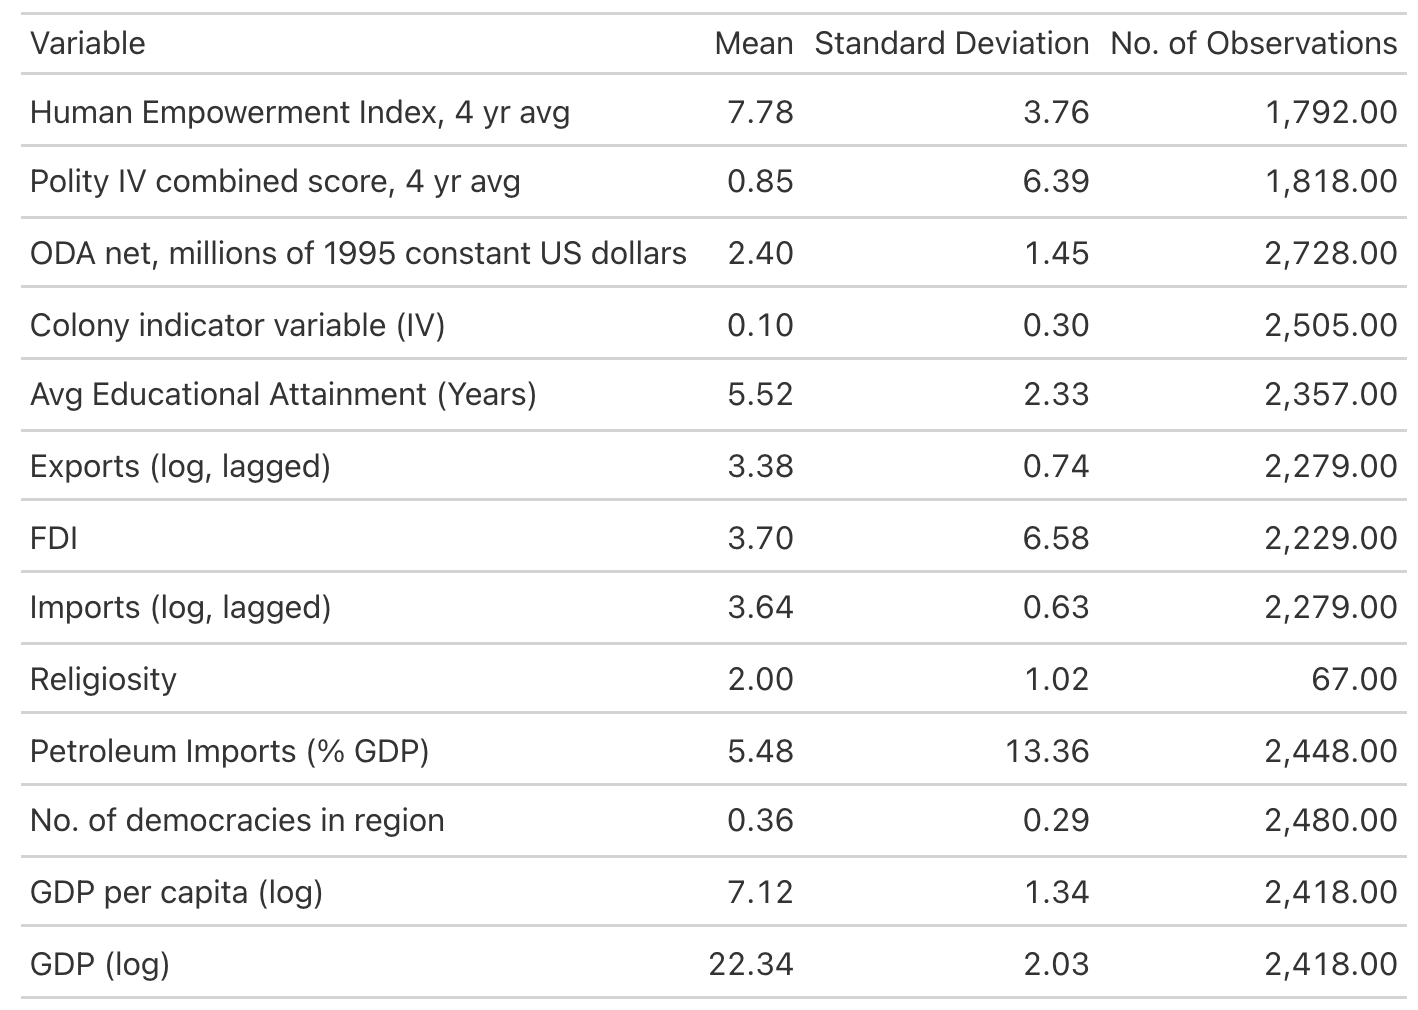
\includegraphics{figures/Table 1.png} \\
\end{longtable}

\hypertarget{results}{%
\section{Results}\label{results}}

I replicate and extend \citet{carnegie2017foreign}'s results below.
First, Table 2 shows the results of the second-stage TSLS specifications
with outcome variables for democracy, human rights, and economic growth
(equations number three and four above). As in
\citet{carnegie2017foreign}, (instrumented) foreign aid has a
statistically significant and positive impact on measures of human
rights and democracy, including after adjusting for covariates and
controlling for country and time fixed effects. In column 1, for
instance, a one unit increase in our first-stage estimate for log ODA in
\(t-1\) leads to a 1.885 increase in the average of the CIRI human
rights index averaged across \(t\) and \(t+3\), holding time and country
invariant characteristics fixed.

In contrast, however, foreign aid has a muted impact on log GDP and log
GDP per capita. Column 5 shows a one unit increase in our first-stage
estimate for log ODA in \(t-1\) leads to a statistically insignificant
-1.69 decrease in log GDP averaged across \(t\) and \(t+3\). Controlling
for other covariates on top of country and time fixed effects changes
this negative impact to -2.96 (column 6), but it is still not
statistically significant. I find a similar story for log GDP per capita
as the outcome variable. In Column 7, we see foreign aid decreases log
GDP per capita by -1.8 units. This estimate is statistically significant
at a p\textless0.10 level. Although only just significant, the effect is
sizable: a 1.8 unit decrease in log GDP per capita is slighly above a
one standard-deviation decrease. This result, together with the size and
direction of coefficients across columns 5-8, provides suggestive
evidence that foreign aid may have a negative effect on some measures of
growth.

\hypertarget{tbl-two}{}
\begin{longtable}[]{@{}l@{}}
\caption{\label{tbl-two}TSLS Estimates of Effects of EU Foreign Aid
(given in year t-1) from the European Community on Dependent Variables
(average measure in years t through t-3)}\tabularnewline
\toprule\noalign{}
\endfirsthead
\endhead
\bottomrule\noalign{}
\endlastfoot
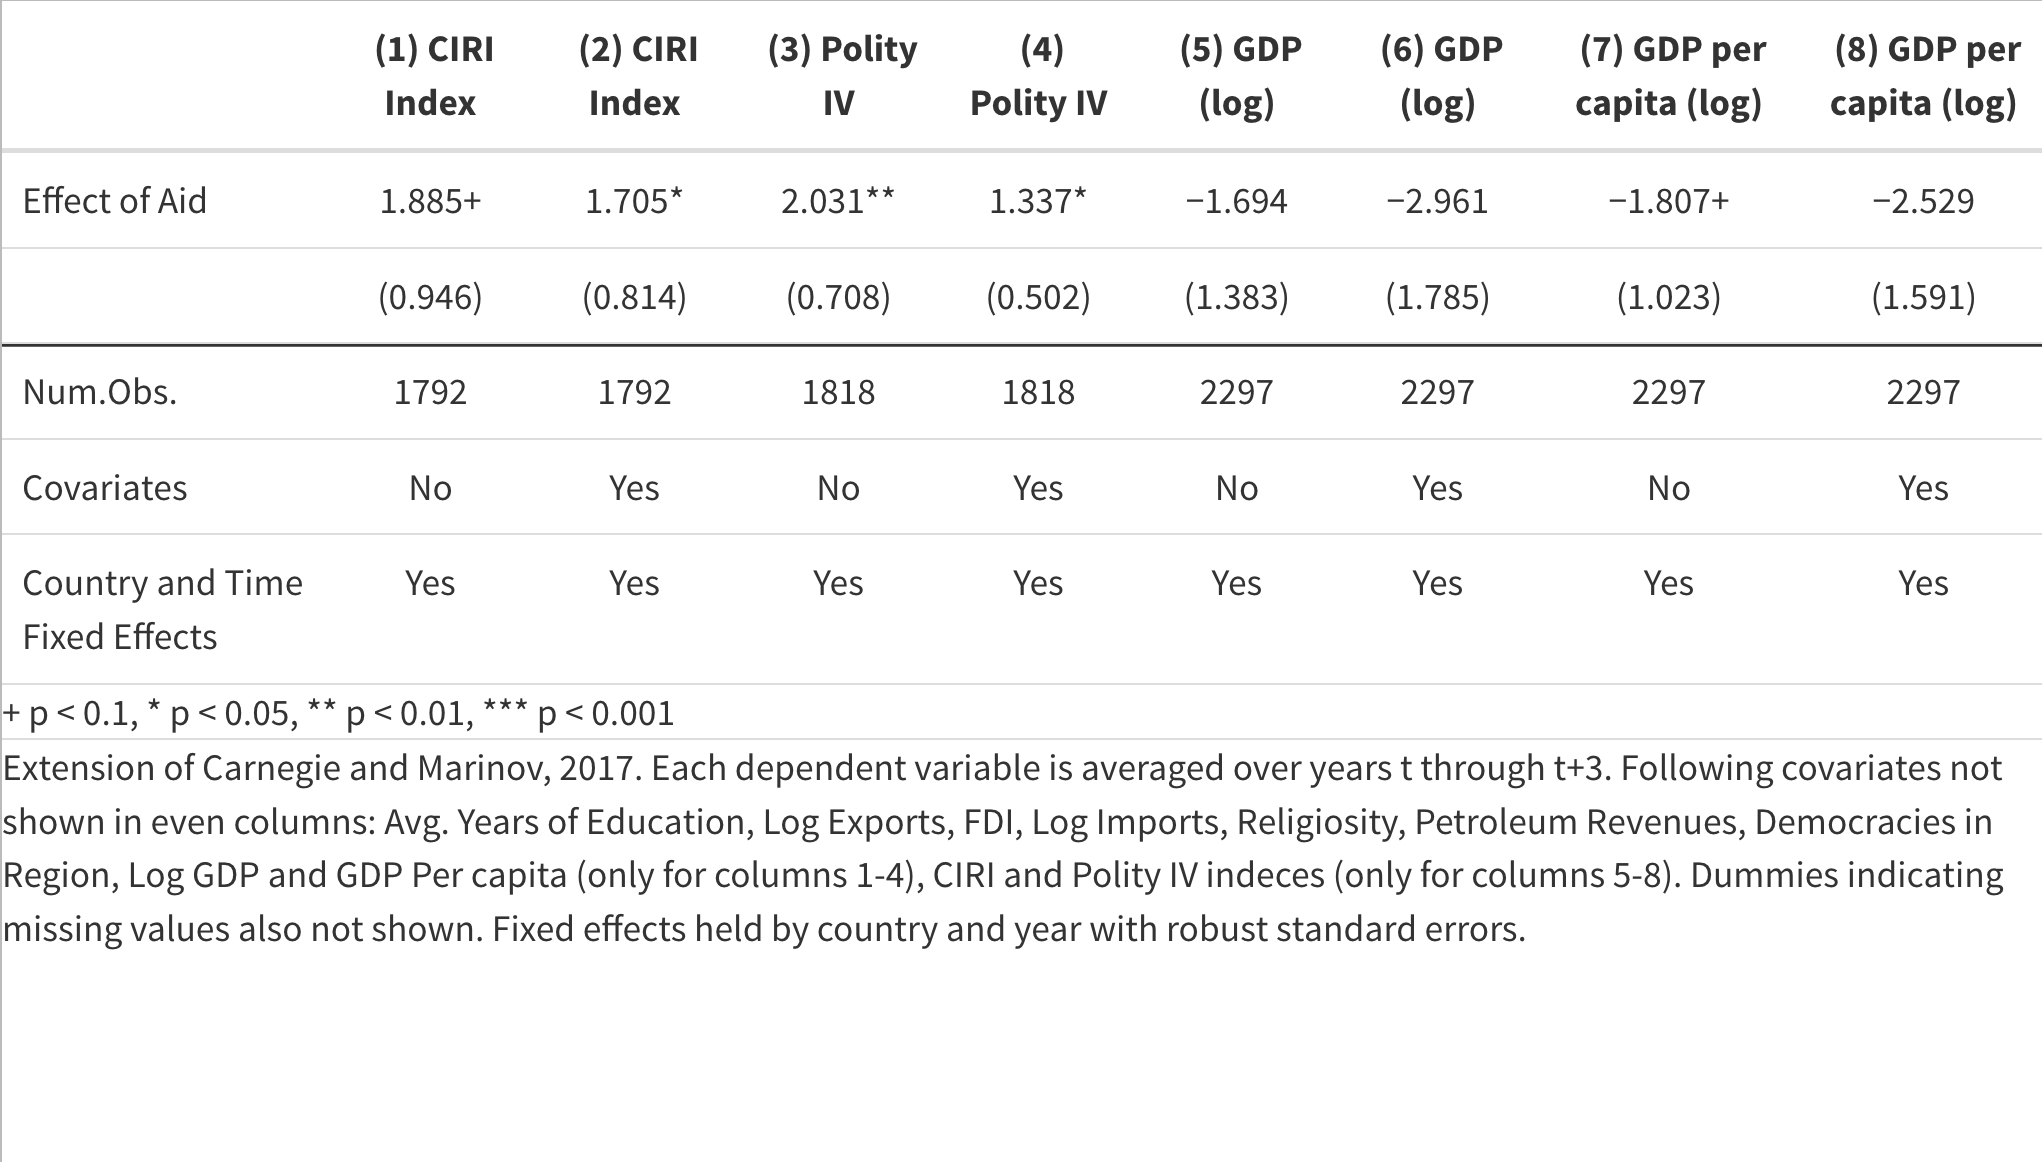
\includegraphics{figures/Table 2.jpeg} \\
\end{longtable}

To determine whether the effects of aid on democracy, human rights, and
growth are short-lived, I replicate and extend
\citet{carnegie2017foreign}'s year-by-year analysis in Figures 1 and 2
below. As in \citet{carnegie2017foreign}, Figure 1 shows that a one unit
increase in our first-stage estimate for log ODA in \(t-1\) leads to
positive and statistically significant increases in CITI (human rights)
at \(t=0\). These effects wear off after \(t=0\) and are no longer
statistically significant by \(t+5\). Looking at Polity IV (democracy),
an increase in ODA first leads to statistically insignificant
improvements in \(t=0\) and \(t+1\), then leads to statistically
significant improvements in \(t + 2\) through \(t+4\), before waning off
and becoming statistically insignificant again by \(t+5\).

\begin{figure}

\begin{minipage}[t]{0.50\linewidth}

{\centering 

\raisebox{-\height}{

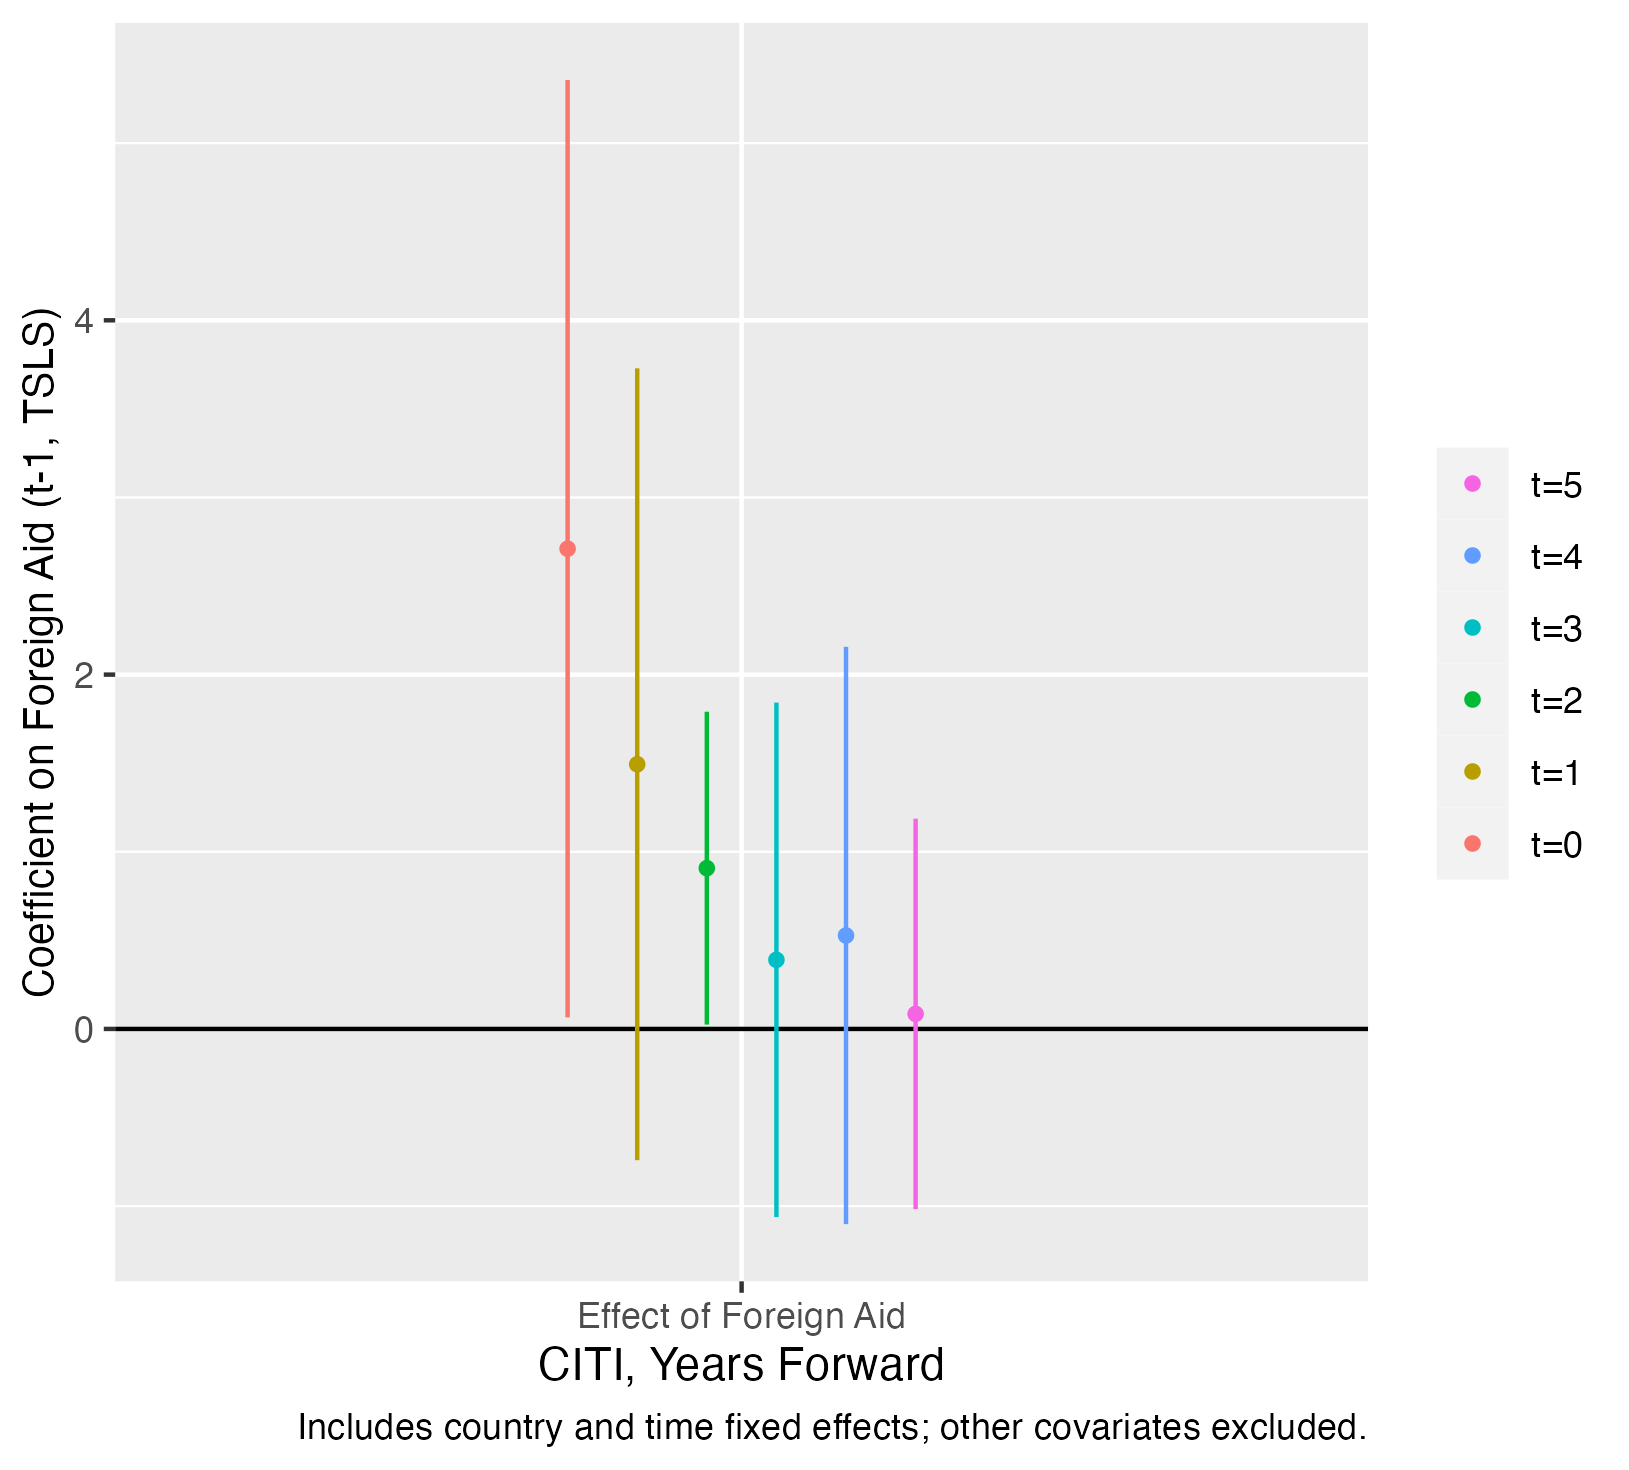
\includegraphics{figures/coefplotCIRI.png}

}

}

\subcaption{\label{fig-citi}CIRI Human Empowerment Index}
\end{minipage}%
%
\begin{minipage}[t]{0.50\linewidth}

{\centering 

\raisebox{-\height}{

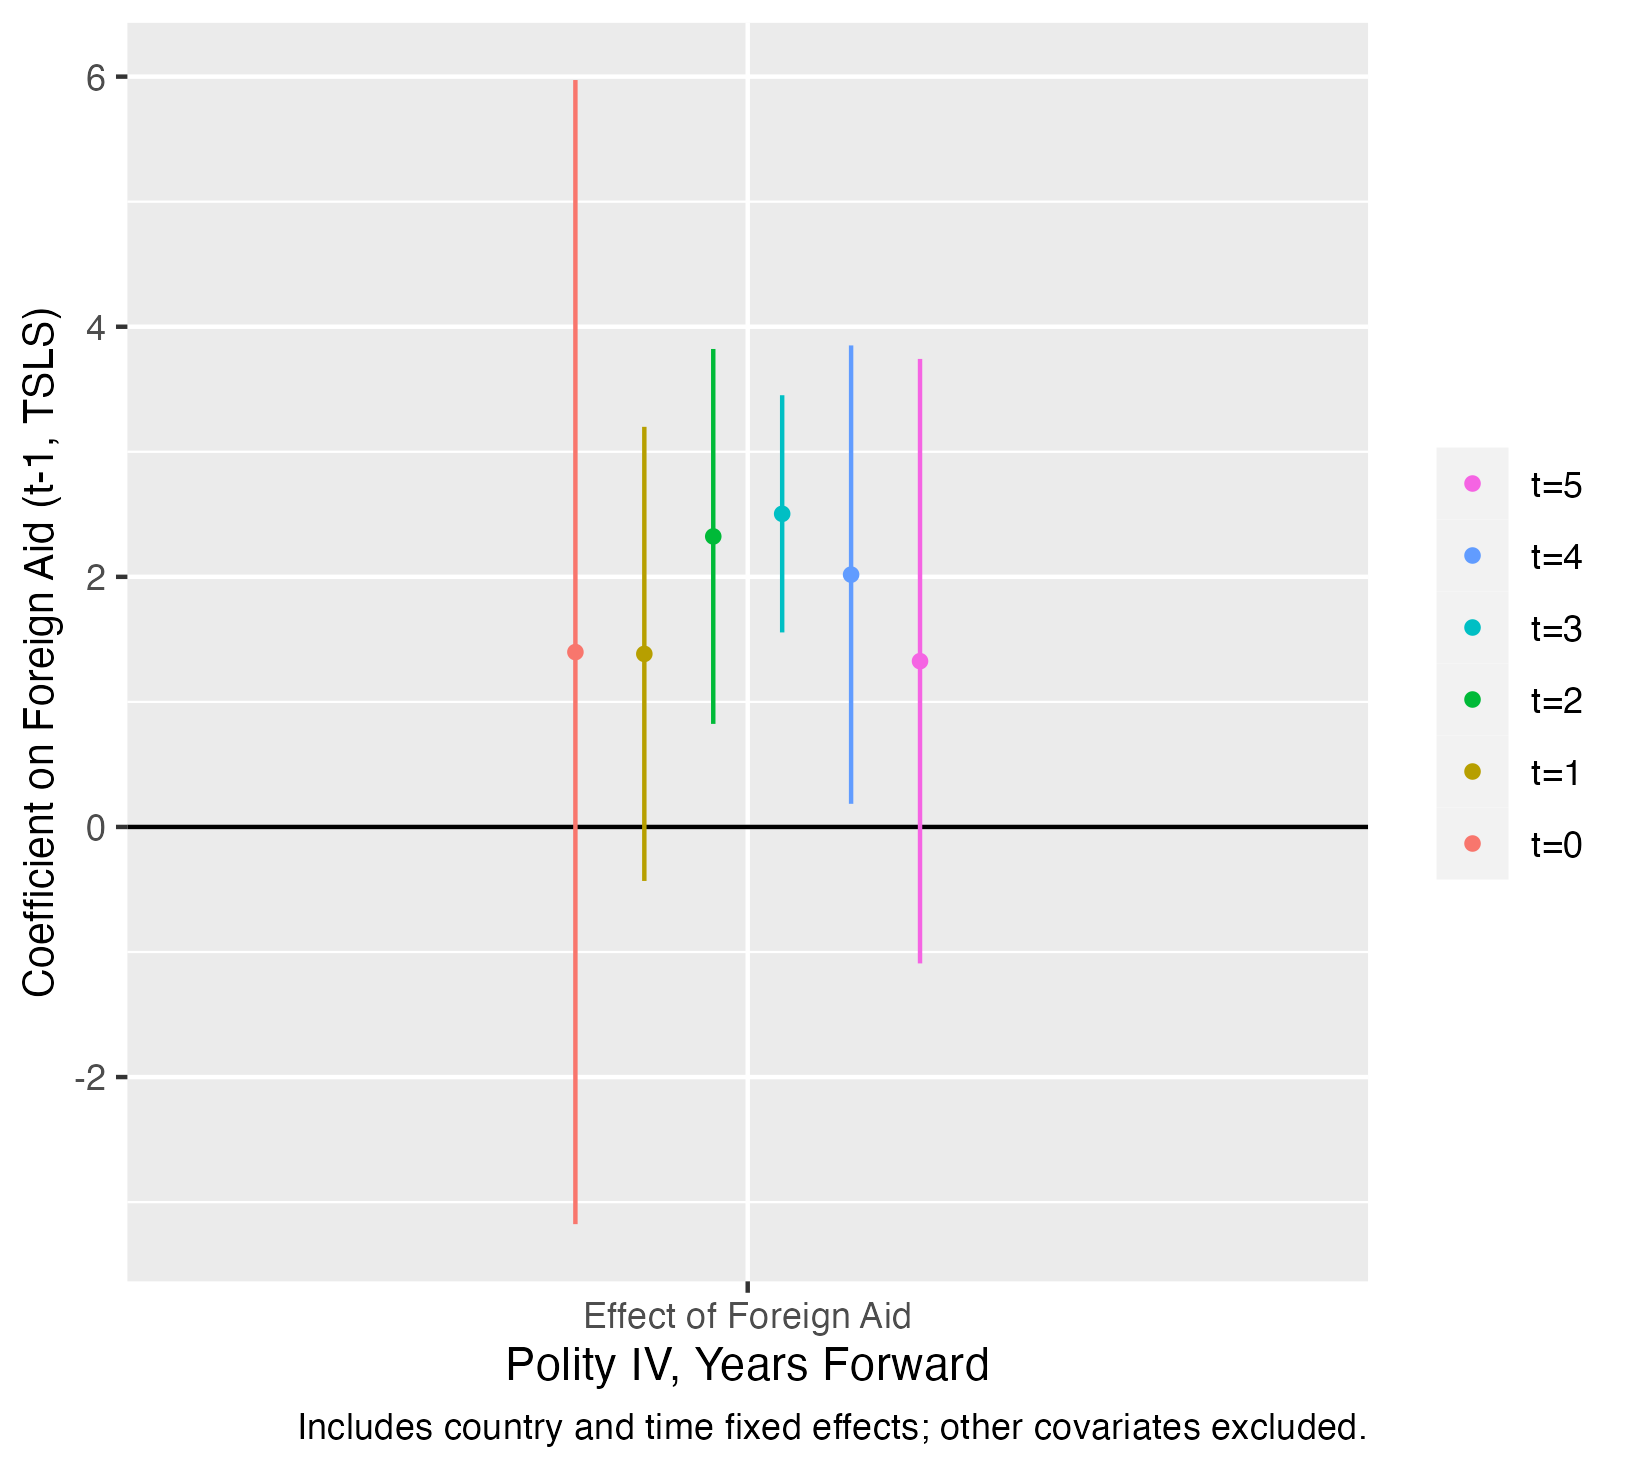
\includegraphics{figures/coefplotPolity.png}

}

}

\subcaption{\label{fig-poly}Polity IV Score}
\end{minipage}%

\caption{\label{fig-replication}Replication of Carnegie and Marinov
(2017): Effects of Foreign Aid (TSLS, given at t-1) on human rights and
democracy measures in later years}

\end{figure}

In contrast to the generally positive (albeit often not statistically
significant) results above, Figure 2 shows foreign aid given at \(t-1\)
has consistently negative results on subsequent-year log GDP and log GDP
per capita measures. The effects of aid on growth are only statistically
significant (and barely so) for log GDP, and only in some years
(\(t=0\), \(t+1\), and \(t+3\)). They are not statistically significant
when log GDP per capita is the outcome variable.

\begin{figure}

\begin{minipage}[t]{0.50\linewidth}

{\centering 

\raisebox{-\height}{

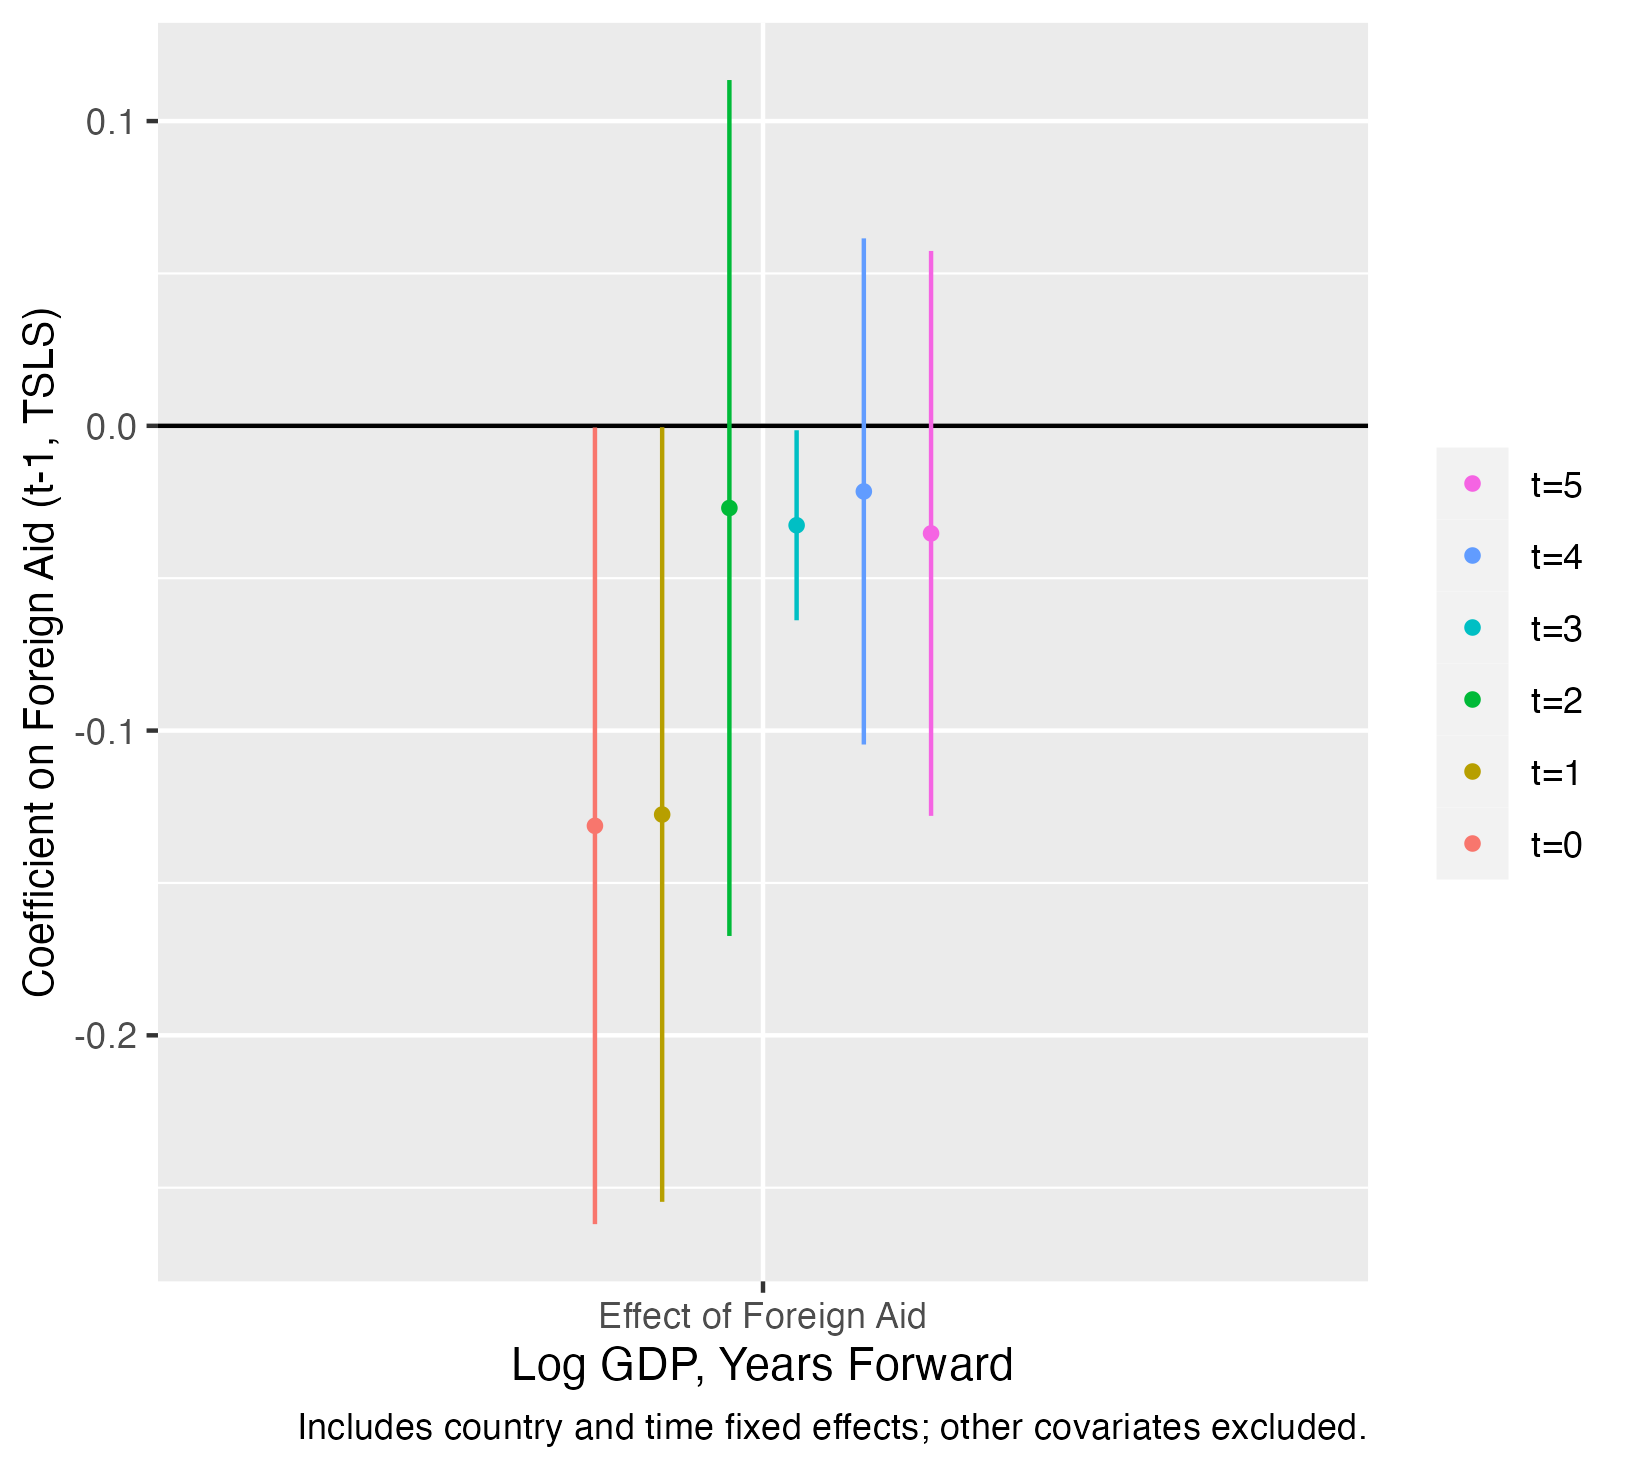
\includegraphics{figures/coefplotLogGDP.png}

}

}

\subcaption{\label{fig-gdp}Log GDP}
\end{minipage}%
%
\begin{minipage}[t]{0.50\linewidth}

{\centering 

\raisebox{-\height}{

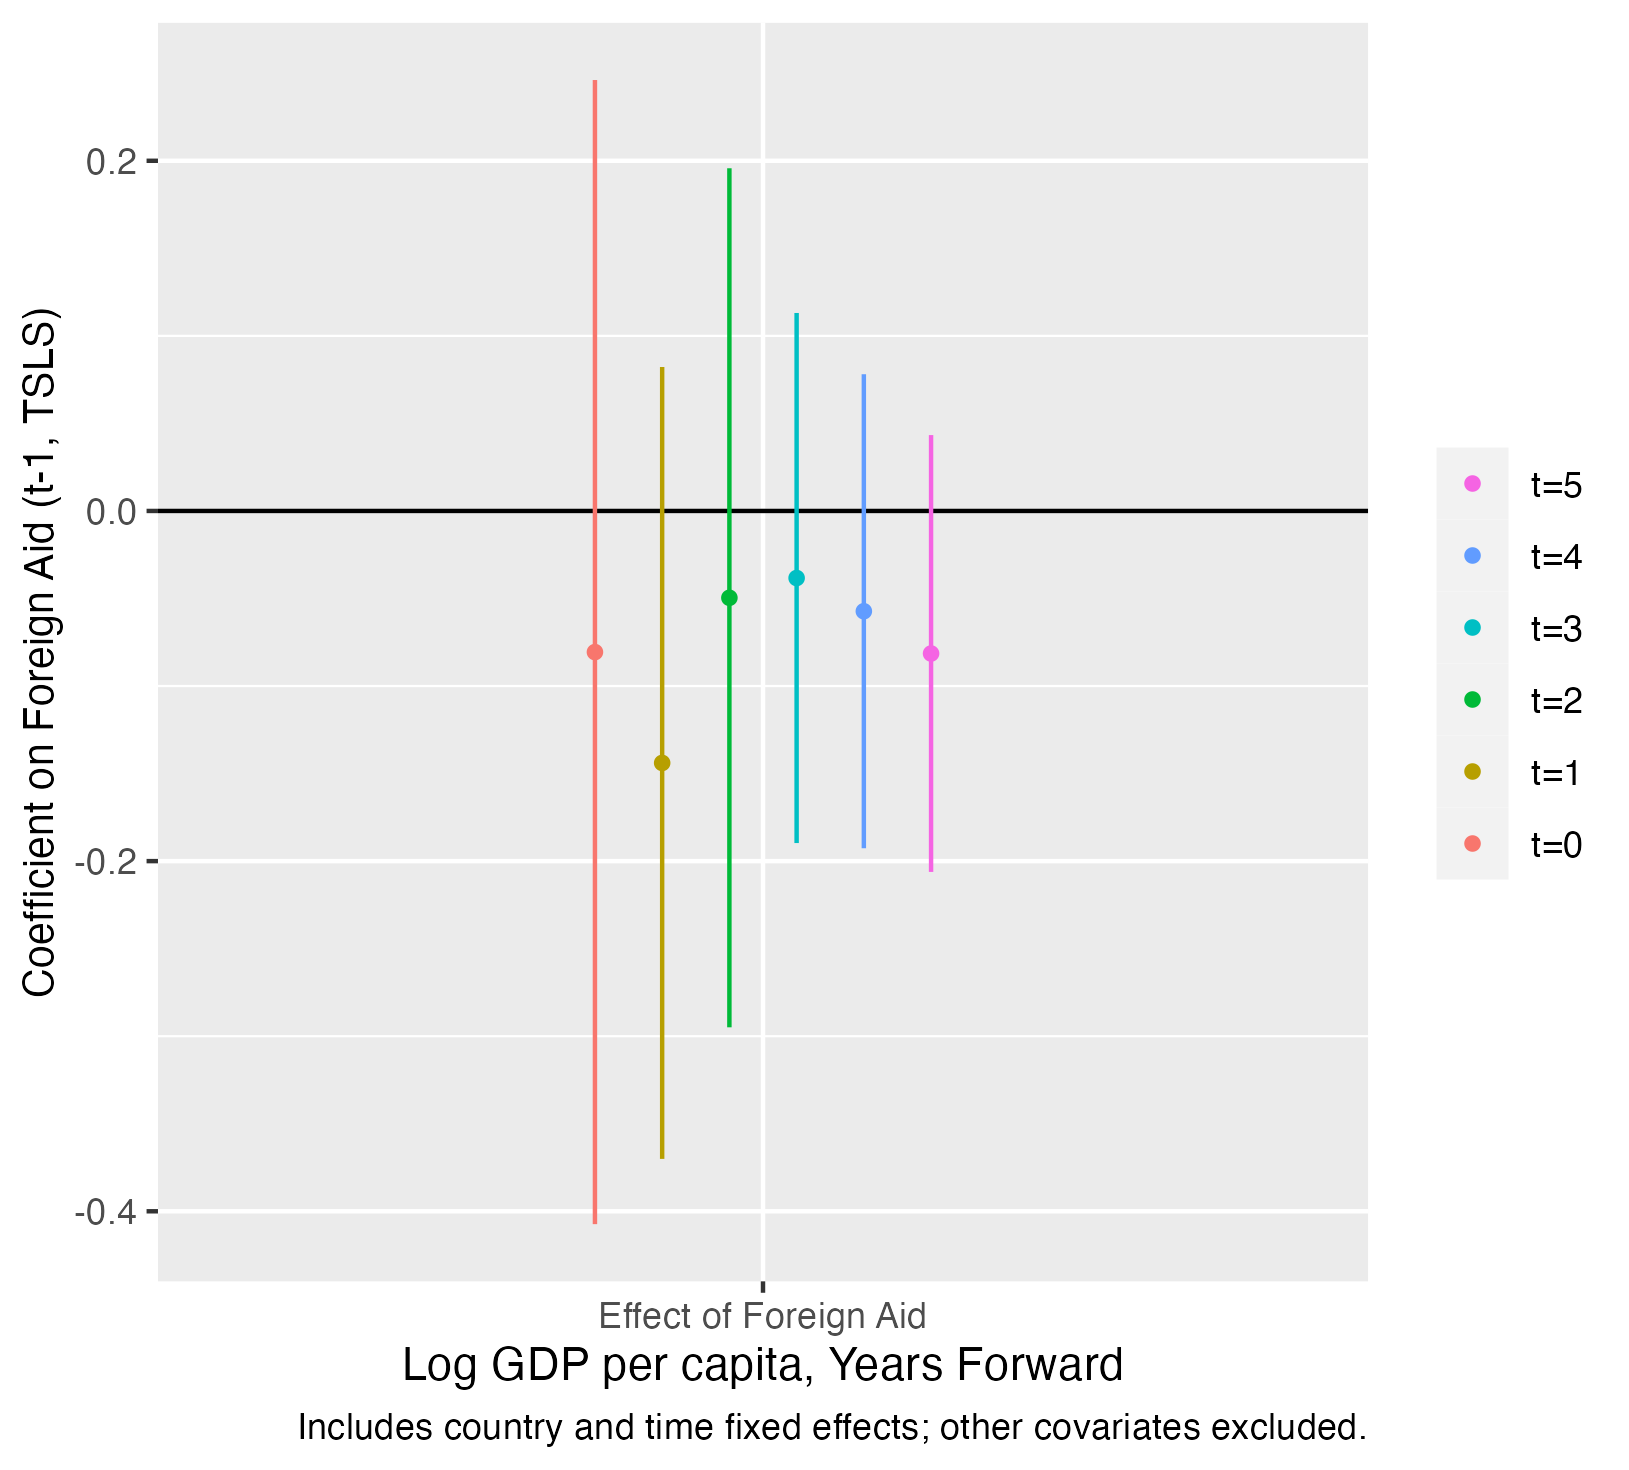
\includegraphics{figures/coefplotLogGDPC.png}

}

}

\subcaption{\label{fig-gdpC}Log GDP per capita}
\end{minipage}%

\caption{\label{fig-extension}Extension of Carnegie and Marinov (2017):
Effects of Foreign Aid (TSLS, given at t-1) on economic growth in later
years}

\end{figure}

\hypertarget{conclusion}{%
\section{Conclusion}\label{conclusion}}

As \citet{carnegie2017foreign} show, EU foreign aid has positive, yet
short-term, effects on recipient countries' measures of democracy and
human rights. In contrast, this aid does not seem to improve recipient
countries' GDP in the short-term. Indeed, there is suggestive evidence
of a negative effect of aid on short-term growth. Leveraging
as-if-random variation from the presidency of the EU Council allowed
\citet{carnegie2017foreign} and I to isolate the causal impact of aid on
these outcomes through an instrumental variables approach.

Other cross-country studies looking at the effect of foreign aid on
economic growth have painted a more positive picture.
\citet{arndt2015what} summarize the findings from multiple studies,
pointing out that they generally find a positive association between aid
and growth. However, they also note that these effects appear to take
place over a longer time horizon. This suggests that the results above
need not be at odds with these other studies, as my analysis only
considers a 5-year time horizon. Future extensions could replicate these
findings over a longer time period, and consider alternative measures of
economic growth beyond GDP and GDP per capita.

\hypertarget{refs}{}

\begin{CSLReferences}{0}{0}\end{CSLReferences}


% END BODY %%%%%%%%%%%%%%%%%%%%%%%%%%%%%%%%%%%%%%%%%%%%%%%%%%%%%%%%%%%%%%%%%%%%%



\end{document}
